\section{Introduction}\label{sec:introduction}

This is a reference to a Section~\ref{sec:related}.

This is a reference to a Figure~\ref{fig:bugra1}.

This is a reference to a Table~\ref{tbl:data}.

This is a bib reference~\cite{ref:SPL}.

\begin{figure*}[t]
\centering
\begin{minipage}{0.48\linewidth}
  \centering
  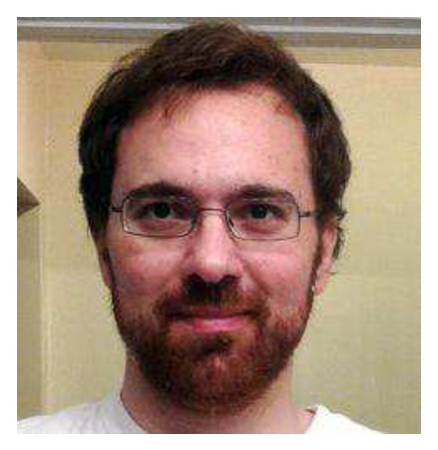
\includegraphics[width=0.5\linewidth]{figures/bugra.eps}
  \caption{Caption goes here}\label{fig:bugra1}
\end{minipage}
\vspace{0.01\linewidth}
\begin{minipage}{0.48\linewidth}
  \centering
  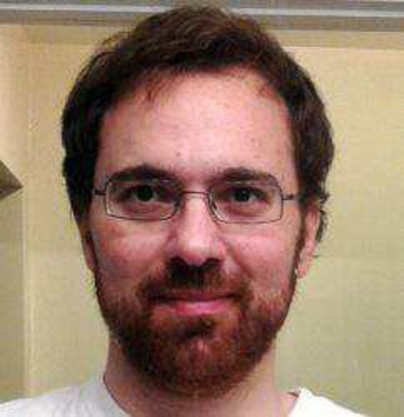
\includegraphics[width=0.5\linewidth]{figures/bugra.pdf}
  \caption{Caption goes here}\label{fig:bugra2}  
\end{minipage}
\end{figure*}


\begin{table*}[t]
\centering
\begin{tabular}{|l||c|c|c|}\hline 
\emph{props.}$\backslash$\emph{names} 
              & seqNo    & RIC     & Date         \\\hline
types         & long     & string  & string       \\\hline
sizes         & $0.08$   & $0.07$  & $0.15$       \\\hline
best alg.     & seq      & zlib    & sameVal      \\\hline
compr. ratios & $\sim 0$ & $0.28$  & $\sim 0$     \\\hline
compr. cost   & $0.006$  & $0.224$ & $0.006$      \\\hline
compr. rank   & $0$      & $7$     & $1$          \\\hline
\end{tabular}
\caption{Properties of the attributes in the TAQ data set.}\label{tbl:data}
\end{table*}            

